\documentclass{book}
\usepackage[utf8]{inputenc}
\usepackage[swedish]{babel}
\usepackage[T1]{fontenc}
\usepackage[utf8]{inputenc}
\usepackage{array}
\usepackage{mathtools}
\usepackage{natbib}
\usepackage{graphicx}
\usepackage{amsfonts}
\usepackage{amsmath}
\usepackage{polynom}
\usepackage{gensymb}
\usepackage{pgfplots} 
\usepackage{tikz}
\usepackage{listings}
\usepackage[top=1in,bottom=1in,right=1in,left=1in]{geometry}
\pgfplotsset{width=10cm,compat=1.9}


\title{Woodworkers handbook on trees}
\author{Anton Augustsson}
\date{June 2020}


\begin{document}

\maketitle
\tableofcontents


\chapter{basic-course-in-mathematics - Formel Samling}

\newpage

\section{Basic}
\subsection{Mängder}
\begin{align*}
  &\quad \text{Naturliga tal: } \mathbb{N} = \{ 1, 2 , 3 ...  \} \\
  &\quad \text{Heltal: }\mathbb{Z} = \{... -2, 1, 0, 1, 2 ...  \} \\
  &\quad \text{Rationella tal: }\mathbb{Q} = \{ \frac{a}{b} | a,b \in \mathbb{Z}, b \\
  &\quad \text{Irrationella tal: }\mathbb{P} = \frac{\mathbb{R}}{\mathbb{Q}}eller \{ x | x \in \mathbb{R}, x \notin \mathbb{Q} \} \\
  &\quad \text{Reella tal: }\mathbb{R} =  \mathbb{P} \cup \mathbb{Q} \\
\end{align*}


\subsection{Potenslagar}
\begin{align*}
  &\quad (\frac{a}{b})^{-3} = (\frac{b}{a})^{3}\\
  &\quad \sqrt{a} = a^{\frac{1}{2}} \\
\end{align*}


\subsection{Logaritmer}
%\begin{align*}
%  &\quad y = a^x \Leftrightarrow \log_a(y) = x  \\
%  &\quad 0<a<1 \text{ och } 1<a \text{ ger olika grafer} \\
%\end{align*}
%
%\begin{tikzpicture}
%\begin{axis}[
%    axis lines = left,
%    xlabel = $x$,
%    ylabel = {$f(x)$},
%]
%%Below the red parabola is defined
%\addplot [
%    domain=-5:5, 
%    samples=100, 
%    color=red,
%]
%{2^x};
%\addlegendentry{$2^x$}
% \addplot [
%    domain=-5:5, 
%    samples=100, 
%    color=black,
%]
%{0.5^x};
%\addlegendentry{$0.5^x$} 
%\end{axis}
%\end{tikzpicture}


\textbf{Logaritmlagar:}\par
Va vaksam över när a<0 då är logarytmen odefinerad. 
\begin{align*}
  &\quad \text{(1): } b = a^x \Leftrightarrow \log_a(b) = x  \text{ för: } a>0, b>0, a \ne 1  \\
  &\quad \text{(2): } \log_a(\frac{b}{c}) = \log_a(b) - \log_a(c) \\
  &\quad \text{(3): } \log_a(b*c) = \log_a(b) + \log_a(c) \\
  &\quad \text{(4): } \log_a(b^d) = d\log_a(b) \\
  &\quad \text{(5): } \log_a(b) = \frac{\log_f(b)}{\log_f(a)} \\
  &\quad \text{(6): } \log_a(a) = 1 \\
  &\quad \text{(7): } \log_a(1) = 0 \\
  &\quad \text{(8): } a^{\log_a(x)} = x \\
  &\quad \text{(9): } \log_{a^c}(b) = \frac{1}{c} \log_a(b) \\
\end{align*}

\subsection{Tillvägagångs sätt}
\begin{equation}
\log_3(x) + \log_x(\frac{1}{27}) = 2
\end{equation}

\subsubsection{Lösning}
\begin{align*}
  &\quad \log_3(x) - 3 \log_x(3) = 2 \\
  &\quad  \log_3(x) - 3 \frac{\log_3(3)}{\log_3(x)} = 2 \\
  &\quad  \log_3(x) - 3 \frac{1}{\log_3(x)} = 2 \\
  &\quad  \log_3(x)^2 - 3 = 2 \log_3(x) \\
  &\quad  y = \log_3(x)^{2} \\
  &\quad  y^2 - 2y- 3 = 0 \\
  &\quad  \text{pq-formeln: } y= 1 \pm \sqrt{4} = 1 \pm 2 \\
  &\quad  \log_3(x) = 3 \Leftrightarrow x = 3^3 = 27 \\
  &\quad  \log_3(x) = -1 \Leftrightarrow x = 3^{-1} = \frac{1}{3} \\
\end{align*}


\subsection{Intervall}
\begin{equation}
[ \, a, b ] \, = \{ x | a \leq x \leq b \}
\end{equation}

\begin{equation}
[ \, a, \infty [ \,
\end{equation}
\begin{equation}
] \, -\infty, \infty [ \,
\end{equation}

\subsection{Tillvägagångs sätt}
\begin{equation}
\frac { 2 } { x - 3 } < \frac { 5 } { x }
\end{equation}


\subsubsection{Lösning}
\begin{align*}
&\quad \frac{ 2 }{ x - 3 } - \frac{ 5 }{ x } < 0 \\
&\quad \frac{(x) 2 }{x (x - 3)} - \frac{ 5 ( x - 3 )}{ x ( x - 3 ) } < 0 \\
&\quad \frac{ 2 x - 5 x - 15 }{ x ( x - 3 ) } < 0 \\
&\quad \frac{ - 3 x - 15 }{ x ( x - 3 ) } < 0 \\
&\quad \frac{ - 3 ( x - 5 ) }{ x ( x - 3 ) } < 0 \\
&\quad  x \neq 0 , x \neq 3 \\
\end{align*}
Värde tabell:
\begin{center}
\begin{tabular}{ |c|c|c|c|c| } 
 \hline
        & x<0   & 0<x<3 & 3<x<5 & 5<x   \\ 
 x-5    & -     & -     & -     & +     \\ 
 -3     & -     & -     & -     & -     \\  
 x      & -     & +     & +     & +     \\ 
 x-3    & -     & -     & +     & +     \\ 
 hela   & +     & -     & +     & -     \\ 
 \hline
\end{tabular}
\end{center}



\section{Komplexa tal}
\begin{align*}
&\quad z = a + bi \\
&\quad \operatorname{Re}(z) = a \\
&\quad \operatorname{Im}(z) = b \\
&\quad \overline{\rm z}= a - b i \\
&\quad | z | = \sqrt{a^ { 2 } + b^ { 2 }} \text{  Där b(Im(z)) är för y-axeln och a(Re(z)) är för x-axeln} \\
&\quad  \\
&\quad \text{Samma räkneregler för reella tal gäller för komplexa tal} \\
\end{align*}


\subsection{Polärform}
\begin{align*}
  &\quad \text{arg}(z) = \alpha + 2\pi * n \\
  &\quad \text{arg(z) är vinkeln mellan a (x-axeln) linjen |z|. n är heltal}  \\
  &\quad \text{Arg}(z) \in ]-\pi, \pi[ \\
    &\quad \text{Arg}(z) \in \text{arg}(z) \\
    &\quad a = |z| \cos{\alpha} \\
    &\quad b = |z| \sin{\alpha} \\
    &\quad z = |z| \cos{\alpha} + i * |z| \sin{\alpha} \\
\end{align*}

\textbf{Polärform:}\par
\begin{equation}
  z = |z|(\cos{\alpha} + i * \sin{\alpha})
\end{equation}

\textbf{Eulers formel:}\par
\begin{equation}
  z = |z|e^{i \alpha}
\end{equation}

\textbf{Sats:}\par
\begin{align*}
  &\quad |z * w| = |z| * |w| \\
  &\quad \text{arg}(z * w) = \text{arg}(z) + \text{arg}(w) \\
  &\quad \text{arg}(\frac{z}{w}) =  \text{arg}(z) - \text{arg}(w)\\
\end{align*}

\newpage

\textbf{De Movre's formel:}\par
\begin{align*}
  &\quad (\cos{(\theta)} + i * \sin{(\theta)})^{n} = \cos{(n*\theta)} + i * \sin{(n*\theta)} \\
\end{align*}


\subsubsection{Binomisk ekvation}
\begin{align*}
  &\quad (\cos{(\theta)} + i * \sin{(\theta)})^{n} = \cos{(n*\theta)} + i * \sin{(n*\theta)} \\
\end{align*}


\subsubsection{Tillvägagångs sätt}
\begin{equation}
  \text{Visa lösningarna i det komplexa tal planet } z^5 = \sqrt{3} + i
\end{equation}

\begin{align*}
  &\quad |\sqrt{3} + i| = \sqrt{\sqrt{3}^2 + 1^2} = \sqrt{4} = 2 \\
  &\quad \left\{ \begin{array} { l } { \sqrt{3} = 2 \cos(\alpha)} \\ { 1 = 2 \sin(\alpha) } \end{array} \right. \\
  &\quad \alpha = \frac{\pi}{6} \\
  &\quad |z|^5(\cos{(5*\theta)} + i * \sin{(5*\theta)}) = 2(\cos{(\frac{\pi}{6})} + i * \sin{(\frac{\pi}{6})}) \\
  &\quad \text{Vilket ger: } \\
  &\quad |z|^5 = 2 \Leftrightarrow |z| = 2^{\frac{1}{5}} \\
  &\quad 5*\theta = \frac{\pi}{6} + 2 \pi n \Leftrightarrow \theta = \frac{\pi}{30} + \frac{2 \pi n}{5} n \in \mathbb{Z} \\
  &\quad \text{I polärform blir det då: } \\
  &\quad z = 2^{\frac{1}{5}} (\cos{\frac{\pi}{30} + \frac{2 \pi n}{5}} + i * \sin{\frac{\pi}{30} + \frac{2 \pi n}{5}}) \\
  &\quad \text{Eulers formel: } z = 2^{\frac{1}{5}} e^{i (\frac{\pi}{30} + \frac{2 \pi n}{5})} \\
  &\quad n = 0,1,2,3,4 \\
  &\quad z_1 = 2^{\frac{1}{5}} e^{i (\frac{\pi}{30})} \\
  &\quad z_2 = 2^{\frac{1}{5}} e^{i (\frac{\pi}{30} + \frac{2 \pi}{5})} \\
  &\quad z_3 = 2^{\frac{1}{5}} e^{i (\frac{\pi}{30} + \frac{4 \pi}{5})} \\
  &\quad z_4 = 2^{\frac{1}{5}} e^{i (\frac{\pi}{30} + \frac{6 \pi}{5})} \\
  &\quad z_5 = 2^{\frac{1}{5}} e^{i (\frac{\pi}{30} + \frac{8 \pi}{5})} \\
\end{align*}

%\begin{figure}
%\begin{tikzpicture}
%[acteur/.style={circle, fill=black,thick, inner sep=2pt, minimum size=0.2cm}
  %\node (a1) at ( 1.3,1.1) [acteur][label=A]{};
%\begin{axis}[
%    xmin=-2.5,
%    xmax=2.5,
%    ymin=-2.5,
%    ymax=2.5,
%    axis equal,
%    axis lines=middle,
%    xlabel=Re($z$),
%    ylabel=Im($z$),
%    disabledatascaling]
%  \fill [opacity=0.3] (0,0) circle [radius=2^(1/5)];
%  \node (a1) at ( 1.3,1.1) [label=z1]{};
%  \filldraw ( 1.3,1.1) circle[radius=1pt];
%  \node (a2) at ( -1.3,1.1) [label=z2]{};
%  \node (a3) at ( -1.3,-1.1) [label=z3]{};
%  \node (a4) at ( 1.3,-1.2) [label=z4]{};
%  \node (a5) at ( 1.8,1.1) [label=z5]{};
%  \draw [-, thick, black] (a1) -- (a2);
%\end{axis}
%\end{tikzpicture}


\newpage
\section{Absolut Belopp}
\subsection{Tillvägagångs sätt}
\begin{equation}
| 2 x - 8 | + | 1 - x | - 2 | x - 3 | = 8 + 3 x
\end{equation}


\subsubsection{lösning}
\begin{align*}
\left( \begin{array} { c } { 2 x - 8 = 0 } \\ { x = 4 } \end{array} \right)
\left( \begin{array} { c } { 1 - x = 0 } \\ { x = 1 } \end{array} \right)
\left( \begin{array} { c } { x - 3 = 0 } \\ { x = 3 } \end{array} \right)
&\quad
&\quad
&\quad
\end{align*}

\begin{align*}
&\quad \text{ I } \left\{ \begin{array} { l } { x \leq 1 } \\ { - ( 2 x - 8 ) + ( 1 - x ) + 2 ( x - 3 ) = 8 + 3 x } \end{array} \right. \\
&\quad \text{ I } \left\{ \begin{array} { l } { x \leq 1 } \\ { - 4 x = 5 } \end{array}  \quad \left\{ \begin{array} { l } { x \leq 1 } \\ { x = - \frac { 5 } { 4 } \text{ lösning}} \end{array} \right. \right. \\
&\quad \text{II } \left\{ \begin{array} { l } { 1 < x \leq 1 } \\ { - ( 2 x - 8 ) - ( 1 - x ) + 2 ( x - 3 ) = 8 + 3 x } \end{array} \right. \\
&\quad \text{II } \left\{ \begin{array} { l } { 1 < x \leq 3 } \\ { - 2 x = 7 } \end{array} \quad \left\{ \begin{array} { l } { 1 < x < 3 } \\ { x = - \frac { 7 } { 2 } \text{ Ej lösning} } \end{array} \right. \right. \\
&\quad \text{III} \left\{ \begin{array} { l } { 3 \leq x < 4 } \\ { - ( 2 x - 8 ) - ( 1 - x ) - 2 ( x - 3 ) = 8 + 3 x } \end{array} \right. \\
&\quad \text{III} \left\{ \begin{array} { l } { 3 \leq x \leq 4 } \\ { - ( 2 x - 8 ) - ( 4 x - 3 ) = 8 + 3 x } \end{array} \quad \left\{ \begin{array} { l } { 3x < 4 } \\ { x = \frac { 5 } { 6 } \text{ Ej lösning} } \end{array} \right. \right. \\
&\quad \text{IV} \left\{ \begin{array} { l } { x \geq 4 } \\ { ( 2 x - 8 ) - ( 1 - x ) - 2 ( x - 3 ) = 8 + 3 x } \end{array} \right. \\
&\quad \text{IV} \left\{ \begin{array} { l } { x \geq 4 } \\ { x = - \frac { 11 } { 2 } \text{ Ej lösning} } \end{array} \right. \\ 
\end{align*}


\newpage

\section{Summor}
\subsection{Aritmetiska summor}
\begin{equation}
s _ { n } = a _ { 1 } + a _ { 2 } + a _ { 3 } + \ldots + a _ { n } = \frac { n \left( a _ { 1 } + a _ { n } \right) } { 2 }
\end{equation}


\subsection{Geometriska summor}
Börjar altid med exponenten 0 och gör om summan så att den passar i följade talföljd:
\begin{equation}
s _ { n } = a + a k + a k ^ { 2 } + \ldots + a k ^ { n - 1 } = \frac { a \left( k ^ { n } - 1 \right) } { k - 1 }
\end{equation}


\subsection{Tillvägagångs sätt}
\begin{equation}
\displaystyle\sum _ { k = n } ^ { 2n } (2^{k} - k)
\end{equation}
\subsubsection{Lösning}
\begin{align*}
  &\quad \text{sätter f = 0 = k -n} \\
  &\quad \displaystyle\sum _ { f = 0 } ^ { n } (2^{f+n} - (f+n)) = 2^{n} * \displaystyle\sum _ { f = 0 } ^ { n } (2^{f}) - \displaystyle\sum _ { f = 0 } ^ { n } (f+n) \\
  &\quad \frac{2^{n} (2^{n+1} -1)}{2-1} - \frac{3n(n+1)}{2} = 2^{2n+1} - 2^{n} - \frac{3n(n+1)}{2}\\
  &\quad  \\
\end{align*}


\newpage

\section{Kombinatorik}
\subsection{Multiplikations principen}
permetationer p(a,b) då ordningen spelar roll. \newline
Antal sätt: (exemplet: antal sätt av måltider 7 företer 5 varmrätter 4 efterätter (7*5*4)
\begin{equation}
n _ { 1 } \cdot n _ { 2 } \cdot \ldots \cdot n _ { m }
\end{equation}


\subsection{Kombinationer}
Kombination c(a,b) då ordningen inte spelar roll. \newline 
Antal sätt: (exemplet: antal del-mängder två element (n = element k = antal element som kan väljas))
\begin{equation}
\left( \begin{array} { l } { n } \\ { k } \end{array} \right) = \frac { n! } { k! (n-k)! }
\end{equation}

\begin{equation}
\left( \begin{array} { l } { n } \\ { k } \end{array} \right) = \frac { n \cdot ( n - 1 ) ( n - 2 ) \cdot \ldots \cdot ( n - 1 ( k - 1 ) ) } { k ! }
\end{equation}


\subsubsection{Pascal triangel}
\begin{center}
\begin{tabular}{>{$}l<{$}|*{7}{c}}
\multicolumn{1}{l}{$n$} &&&&&&&\\\cline{1-1} 
0 &1&&&&&&\\
1 &1&1&&&&&\\
2 &1&2&1&&&&\\
3 &1&3&3&1&&&\\
4 &1&4&6&4&1&&\\
5 &1&5&10&10&5&1&\\
6 &1&6&15&20&15&6&1\\\hline
\multicolumn{1}{l}{} &0&1&2&3&4&5&6\\\cline{2-8}
\multicolumn{1}{l}{} &\multicolumn{7}{c}{$k$}
\end{tabular}
\end{center}


\subsection{Binomial satsen}
\begin{equation}
(a + b)^{n} = \displaystyle\sum _ { k = 0 } ^ { n } \left( \begin{array} { l } { n } \\ { k } \end{array} \right) a ^ {k} b ^ { n - k }
\end{equation}


\newpage

\section{Funktioner och kordinatsystem}
Kom ihåg att när det stor (x-a) förflytas den i x-axeln a steg till höger --> medans (x+a) förflytas den a steg till vänster <-- 
\subsection{Avståndsformeln}
\begin{equation}
d = \sqrt { \left( x _ { 2 } - x _ { 1 } \right) ^ { 2 } + \left( y _ { 2 } - y _ { 1 } \right) ^ { 2 } }
\end{equation}


\subsection{Elipser}
Förenkla till denna formeln:
\begin{equation}
\frac { x ^ { 2 } } { a ^ { 2 } } + \frac { y ^ { 2 } } { b ^ { 2 } } = 1
\end{equation}
Där a är avståndet på x-axeln och b är avståndet på y-axeln


\subsubsection{Hyperbol}
Ser väldigt anerlunda ut från elipser
\begin{equation}
\frac { x ^ { 2 } } { a ^ { 2 } } - \frac { y ^ { 2 } } { b ^ { 2 } } = 1
\end{equation}


\subsubsection{Circkel}
\begin{equation}
\frac { x ^ { 2 } } { a ^ { 2 } } + \frac { y ^ { 2 } } { a ^ { 2 } } = 1
\end{equation}
Där a = r


\newpage

\section{Polynom division}
\subsection{Tillvägagångs sätt}
\begin{equation}
   \text{Man vet att ekvationen} z^4 - 2z^3 - 7z^2 + 26z - 20 = 0 \text{ har roten } z = 2 + i \text{. Lös ekvationen fullständigt.}
\end{equation}
\begin{align*}
  &\quad z = 2 + i \text{ Är en läsning är också konjugatet en lösning enligt faktorsatsen } \overline{\rm z}= a - b i \\
  &\quad z = 2 \pm i \\
  &\quad \text{Vilket betyder att följande går att factorisera ut polynomet} \\
  &\quad (z -(2 + i))(z -(2 - i)) = z^2 - 4z + 5 \\
\end{align*}

\textbf{Långdivition (liggande stolen):}\par
\polylongdiv[style=A]{x^{4}-2x^{3}-7x^{2}+26x-20}{x^{2}-4x+5}%{x ^ { 3 } - 3 x ^ { 2 } - 6 x + 8}{x-1}%{6x^3-2x^2+x+3}{x^2-x+1}

\begin{align*}
  &\quad z^2 + 2z - 4 = 0 \text{ Är också en läsning som tilslut ger följande} \\
  &\quad z = -1 \pm \sqrt{5} \\
  &\quad z = 2 \pm i \\
  &\quad \text{Varge n grads polynom har altid n stycken komplexa lösningar} \\
\end{align*}


\newpage

\section{Trigonometri}
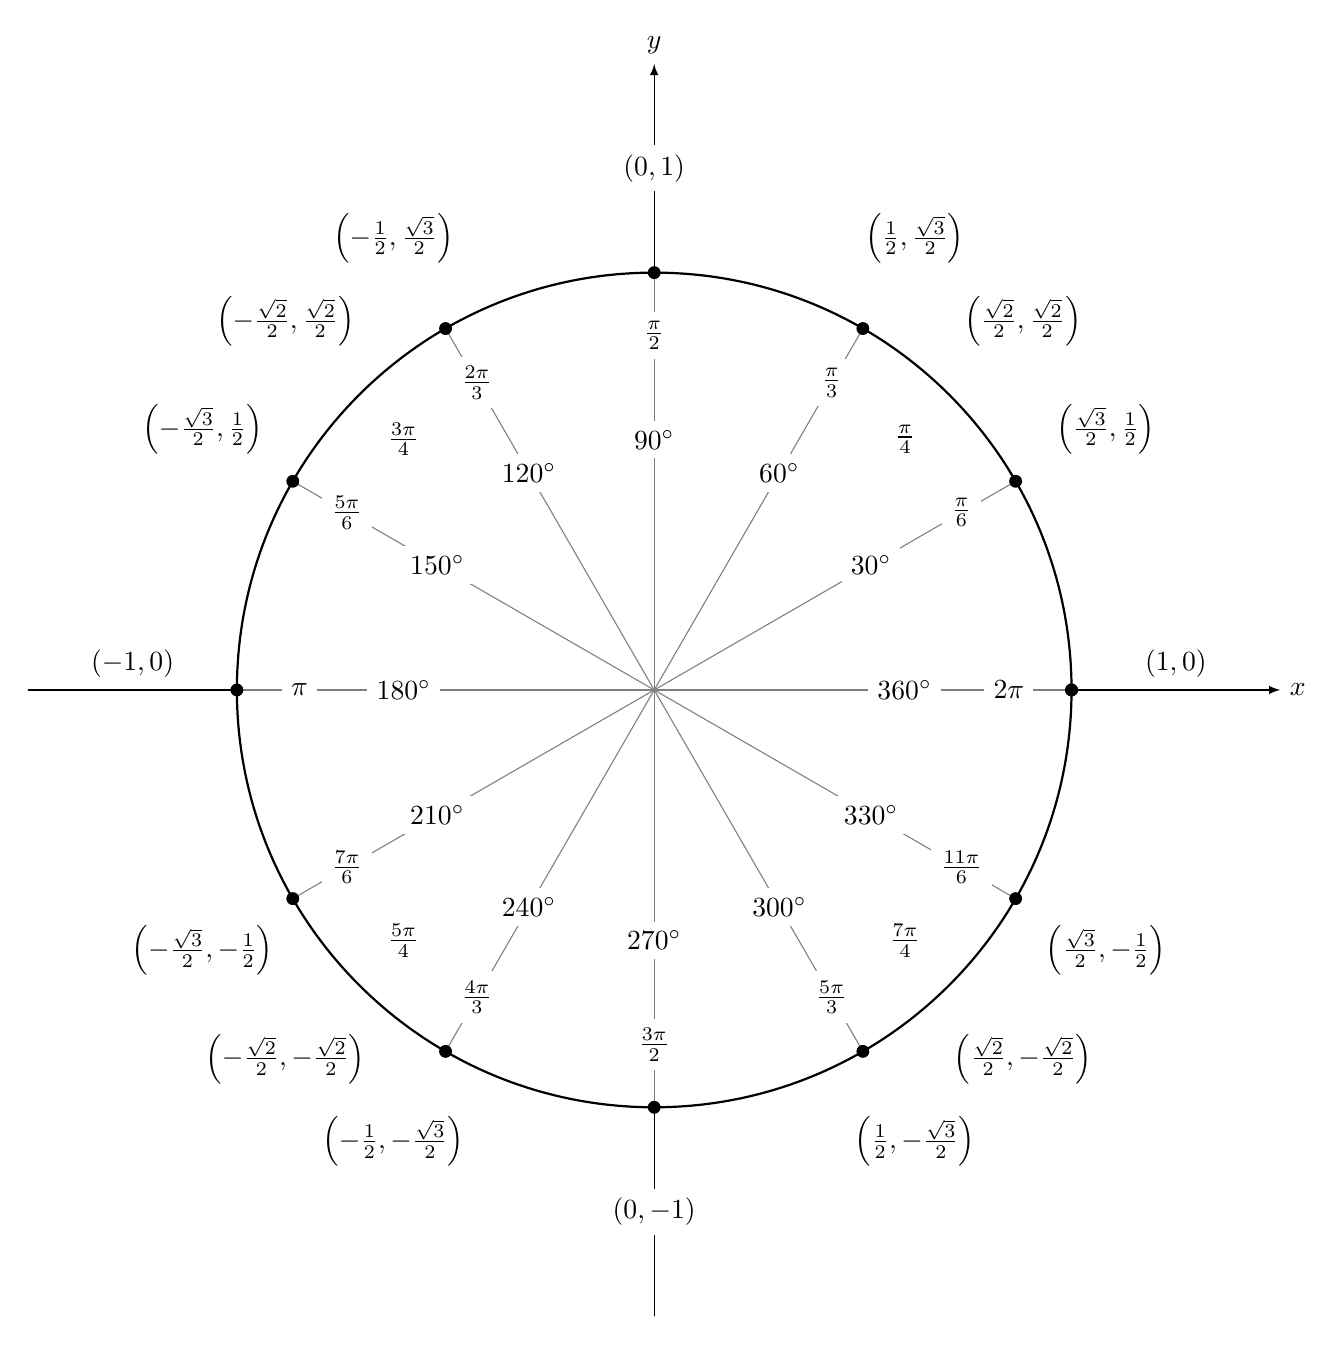
\begin{tikzpicture}[scale=5.3,cap=round,>=latex]
        % draw the coordinates
        \draw[->] (-1.5cm,0cm) -- (1.5cm,0cm) node[right,fill=white] {$x$};
        \draw[->] (0cm,-1.5cm) -- (0cm,1.5cm) node[above,fill=white] {$y$};

        % draw the unit circle
        \draw[thick] (0cm,0cm) circle(1cm);

        \foreach \x in {0,30,...,360} {
                % lines from center to point
                \draw[gray] (0cm,0cm) -- (\x:1cm);
                % dots at each point
                \filldraw[black] (\x:1cm) circle(0.4pt);
                % draw each angle in degrees
                \draw (\x:0.6cm) node[fill=white] {$\x^\circ$};
        }

        % draw each angle in radians
        \foreach \x/\xtext in {
            30/\frac{\pi}{6},
            45/\frac{\pi}{4},
            60/\frac{\pi}{3},
            90/\frac{\pi}{2},
            120/\frac{2\pi}{3},
            135/\frac{3\pi}{4},
            150/\frac{5\pi}{6},
            180/\pi,
            210/\frac{7\pi}{6},
            225/\frac{5\pi}{4},
            240/\frac{4\pi}{3},
            270/\frac{3\pi}{2},
            300/\frac{5\pi}{3},
            315/\frac{7\pi}{4},
            330/\frac{11\pi}{6},
            360/2\pi}
                \draw (\x:0.85cm) node[fill=white] {$\xtext$};

        \foreach \x/\xtext/\y in {
            % the coordinates for the first quadrant
            30/\frac{\sqrt{3}}{2}/\frac{1}{2},
            45/\frac{\sqrt{2}}{2}/\frac{\sqrt{2}}{2},
            60/\frac{1}{2}/\frac{\sqrt{3}}{2},
            % the coordinates for the second quadrant
            150/-\frac{\sqrt{3}}{2}/\frac{1}{2},
            135/-\frac{\sqrt{2}}{2}/\frac{\sqrt{2}}{2},
            120/-\frac{1}{2}/\frac{\sqrt{3}}{2},
            % the coordinates for the third quadrant
            210/-\frac{\sqrt{3}}{2}/-\frac{1}{2},
            225/-\frac{\sqrt{2}}{2}/-\frac{\sqrt{2}}{2},
            240/-\frac{1}{2}/-\frac{\sqrt{3}}{2},
            % the coordinates for the fourth quadrant
            330/\frac{\sqrt{3}}{2}/-\frac{1}{2},
            315/\frac{\sqrt{2}}{2}/-\frac{\sqrt{2}}{2},
            300/\frac{1}{2}/-\frac{\sqrt{3}}{2}}
                \draw (\x:1.25cm) node[fill=white] {$\left(\xtext,\y\right)$};

        % draw the horizontal and vertical coordinates
        % the placement is better this way
        \draw (-1.25cm,0cm) node[above=1pt] {$(-1,0)$}
              (1.25cm,0cm)  node[above=1pt] {$(1,0)$}
              (0cm,-1.25cm) node[fill=white] {$(0,-1)$}
              (0cm,1.25cm)  node[fill=white] {$(0,1)$};
\end{tikzpicture}

\newpage

\textbf{Sats:}\par
\begin{align*}
  &\quad 360^\circ = 2\pi rad \\
  &\quad v_{g} = v_{r} * \frac{180^\circ}{\pi} \\
  &\quad v_{r} = v_{g} * \frac{\pi}{180^\circ} \\
\end{align*}

\textbf{Sats:}\par
\begin{align*}
  &\quad -1 \leq \sin{t} \leq 1 \\
  &\quad -1 \leq \cos{t} \leq 1 \\
\end{align*}

\textbf{Sats:}\par
\begin{align*}
  &\quad \cos{(-t)} = \cos{(t)} \\
  &\quad \sin{(-t)} = -\sin{(t)} \\
  &\quad \tan{(-t)} = \frac{\sin{(-t)}}{\cos{(-t)}} = \frac{-\sin{(t)}}{\cos{(t)}} \\
\end{align*}

\textbf{Additionsformlerna:}\par
\begin{align*}
  &\quad \sin{(\alpha + \beta)} = \sin{(\alpha)}\cos{(\beta)} + \sin{(\beta)}\cos{(\alpha)} \\
  &\quad \sin{(\alpha - \beta)} = \sin{(\alpha)}\cos{(\beta)} - \sin{(\beta)}\cos{(\alpha)} \\
  &\quad \cos{(\alpha + \beta)} = \cos{(\alpha)}\cos{(\beta)} - \sin{(\beta)}\sin{(\alpha)} \\
  &\quad \cos{(\alpha - \beta)} = \cos{(\alpha)}\cos{(\beta)} + \sin{(\beta)}\sin{(\alpha)} \\ 
\end{align*}

\textbf{Trigonometriska ettan:}\par
\begin{align*}
  &\quad (\sin{t})^{2} + (\cos{t})^{2} = 1 \\
  &\quad \sin^{2}{t} + \cos^{2}{t} = 1 \\ 
\end{align*}


\subsection{Tillvägagångs sätt}
\begin{align*}
  \begin{aligned} \cos \frac { \pi } { 12 } & = \cos \left( \frac { \pi } { 3 } - \frac { \pi } { 4 } \right) = \cos \frac { \pi } { 3 } \cos \frac { \pi } { 4 } + \sin \frac { \pi } { 3 } \sin \frac { \pi } { 4 } \\ & = \left( \frac { 1 } { 2 } \right) \left( \frac { 1 } { \sqrt { 2 } } \right) + \left( \frac { \sqrt { 3 } } { 2 } \right) \left( \frac { 1 } { \sqrt { 2 } } \right) = \frac { 1 + \sqrt { 3 } } { 2 \sqrt { 2 } } \end{aligned}
\end{align*}
 \newpage
\chapter{Program Design and Data Structures}

\newpage


\begin{multicols}{2}
\section{Coding convension}
\noindent\textbf{VARIANT} \newline
A (recursive) function terminates if it has a variant.
The variant need to follow all of the flowing rules

\begin{itemize}
\item Needs to decrease every recursive call
\item All ways positive
\end{itemize} 

\noindent\textbf{Side effects} \newline
All IO functions have side effects in order to separate pure Haskell function with impure functions
that changes the state with is commonly the case with imperative and object oriented programming.
Every IO function has a side effects.

\noindent\textbf{INVARIANT} \newline
A data types invariant is what value are allowed for the data type to work. Similar to preconditions for
a function. An example is integer data type that can only use positive integers therefor the
invariant is positive integers.



\section{Design approach}
\begin{itemize}
\item top-down design (Cheating): Is to break down a complex system in to subsystems to solve the problem.
  Most often is to write everything by scratch.
\item bottom-up design (Stacking): Is to piece existing system together to create a more complex system.
  little is programmed, most is copied.
\item dodging: Get some code working more quickly, make progress with some part of the system
  and back-paddle to the dodged part later. The reason is to develop insight that will help solve
  the larger problem.
\end{itemize}


\subsection{Process}
\begin{enumerate}
\item  Data Description
\item  Data Examples
\item  Function Description
\item  Function Examples
\item  Function Template
\item  Code
\item  Tests
\item  Review and Refactor
\end{enumerate}

\noindent\textbf{Programming to an Interface}
More dynamic, can change models, less code to write and a layer of abstraction. ADT 


\section{Recursion}
\subsection{Recursion types}
\begin{enumerate}
\item Simple recursion: There is at most one recursive call (in each branch)
  and the argument is decremented by one.
\item Complete recursion: Some argument becomes smaller in the recursive call, but not necessarily.
\item Multiple recursion: There are multiple recursive calls (in the same branch).
\item Mutual recursion: Two or more functions are defined in terms of each other.
\item Nested recursion: An argument to a recursive call is computed by a recursive call.
\item Recursion on a generalized problem: Sometimes, no suitable recursion scheme is obvious.
\end{enumerate}


\section{Complexity}
\subsection{Growth}
\begin{enumerate}
\item Big $ \theta $ Notation: estimate of growth in intervals determine by constants
  Definition
  For non-negative functions f and g, $f (n) = \theta (g (n))$ if and only if there
  exist $ n_0 \geq 0 $ and $ c_1 , c_2 > 0 $ such that for all $ n > n_0 $
  $ c_1 \cdot g (n) \leq f (n) \leq c_2 \cdot g (n) $.
  $ \theta (g (n)) $ is the set of all functions $ f(n) $ that are bounded below and above
\item Big $ \Omega $ Notation: estimate of growth Lower bound
\item Big $ O $: Notation: estimate of growth upper bound
\end{enumerate}


\subsubsection{Relation}
$O(g(n)) \cap \omega (g(n)) = \theta (g(n))$


\section{Recurrences}
\noindent\textbf{Example:} \newline
sumList $[]$ = 0 \newline
sumList (x:xs) = x + sumList xs

\begin{enumerate}
\item pattern matching $[]$ takes $t_0$ time
\item pattern matching $(x:xs)$ takes $t_1$ time
\item Adding x with recursive call takes $t_{add}$
\item Then the recursive call takes $T(n-1)$
\end{enumerate}

\[ T(n) =
  \begin{cases}
    t_0                   & \quad \text{if } n = 0 \\
    T(n-1)+t_{add} +t_{1}  & \quad \text{if } n > 0 
  \end{cases}
\]


\subsection{Closed Form}
\noindent\textbf{1. Use the substitution method to obtain a closed form for the following recurrence:}
\begin{align*}
  &\quad  f(0) = 5 \\
  &\quad  f(n) = f(n -1) + n + 2, n> 0 \\
\end{align*}
\textbf{Hint: $1 + 2 + 3 + · · · + n = \frac{n(n+1)}{2}$ — you do not need to prove this fact.}


\subsubsection{Expansion Method}
\begin{flalign*}
  & f(0) = 5 \\
  & f(1) = f(0) +n +2 = n +5 +2 \\
  & f(2) = f(1) +n +2 = 2n +5 +2 +2 \\
  & f(3) = f(2) +n +2 = 3n +5 +2 +2 +2 \\
  & f(n) = +n^2 +5 +n \cdot 2 \\
\end{flalign*}
\end{multicols}
\raggedcolumns

\noindent\textbf{Induction proof}
\begin{align*}
  &\quad  \text{Step1: test with base case sense the base case is predefine for 0 we do } n=1  \\
  &\quad  {f(1)}_{VL} = 1^2 +5 +1 \cdot 2 = 8, \\
  &\quad  {f(1)}_{HL} = f(0) +1 +2 = 5 +3 = 8 \\
  &\quad  {f(1)}_{VL} = {f(1)}_{HL} \\
  &\quad  \\
  &\quad  \text{Step2: assumption for p } f(p) = p^2 +5 +p \cdot 2 \\
  &\quad  {f(p+1)}_{VL} = f(p) +(p+1) +2 = (p^2 +5 +p \cdot 2) +(p+1) +2 = \\
  &\quad  = (p^2 +(p+1)) +5 +(p+1) \cdot 2 = (p^2+2p+1) +5 +(p+1) \cdot 2 \\
  &\quad  {f(p+1)}_{HL} = (p+1)^2 +5 +(p+1) \cdot 2 = (p^2+2p+1) +5 +(p+1) \cdot 2 \\
  &\quad  {f(p+1)}_{VL} = {f(p+1)}_{HL} \\
  &\quad  \\
  &\quad  \text{Conclusion: according to induction hypothesis the recurrence of the function is equal to } \\
  &\quad  2n + 5 + \frac{n(1+n)}{2} 
\end{align*}


\subsubsection{Substitution Method}
\begin{align*}
  f(n) &\quad = f(n-1) + n + 2  \\
  &\quad = (f(n-2) + (n-1) + 2) +1n +2 \\               &\quad = f(n-2) + (n-1) + n +2 \cdot 2 \\
  &\quad = (f(n-3) + (n-2) + 2) (n-1) + n +2 \cdot 2 \\ &\quad = f(n-3) +(n-2) + (n-1) + n +3 \cdot 2 \\
  &\quad . \\
  &\quad = f(n-k) + (n -(k-1)) + (n -(k-2)) + (n -(k-3)) + \ldots + n +k \cdot 2  \\
  &\quad . \\
  &\quad = f(n-n) + (n -(n-1)) + (n -(n-2)) + (n -(n-3)) + \ldots + n +n \cdot 2 \\
  &\quad = f(0) +1 +2 +3 + \ldots + n +n \cdot 2 = 5 +1 +2 +3 + \ldots + n +n \cdot 2\\
\end{align*}

We can see the following patterns
\begin{align*}
  &\quad 2n + 5 + \displaystyle\sum_{k=1}^{n}(k) = 2n + 5 + \frac{n(1+n)}{2} \\
\end{align*}

\noindent\textbf{Induction proof}
\begin{align*}
  &\text{Step1: test with base case since the base case is predefine for 0 we do } n=1  \\
  {f(1)}_{VL} &= 2 \cdot 1 + 5 + \frac{1(1+1)}{2} = 2 +5 +1 = 8, \\
  {f(1)}_{HL} &= f(0) + 1 +2 = 5 +3 = 8 \\
  {f(1)}_{VL} &= {f(1)}_{HL} \\
  &\\
  &\text{Step2: assumption for p } f(p) = 2p + 5 + \frac{p(1+p)}{2} \\
  {f(p+1)}_{HL} &= f(p) +(p+1) +2 = (2p +5 +\frac{p(1+p)}{2}) + (p+1) + 2 = \\
  &= 2(p+1) +5 +\frac{p(1+p)}{2} +p = 2(p+1) +5 +\frac{2(p+1)+p(1+p)}{2} = \\
  &= 2(p+1) +5 +\frac{p^2 +2p +p +2}{2} = \\
  {f(p+1)}_{HL} &= 2(p+1) + 5 + \frac{(p+1)(p+2)}{2} = 2(p+1) + 5 + \frac{p^2 +2p +p +2}{2}  \\
  {f(p+1)}_{VL} &= {f(p+1)}_{HL} \\
  &\\
  &\text{Conclusion: according to induction hypothesis the recurrence of the function is equal to } \\
  &2n + 5 + \frac{n(1+n)}{2} 
\end{align*}


\newpage
\section{Higher-Order Function}
\subsection{Higher-Order Functions on Lists}
\begin{center}
\begin{tabular}{c}
\begin{lstlisting}[language=Haskell]
map :: (a -> b) -> [a] -> [b]
filter :: (a -> Bool) -> [a] -> [a]
foldl :: (a -> b -> a) -> a -> [b] -> a
foldr :: (a -> b -> b) -> b -> [a] -> b  
\end{lstlisting}
\end{tabular}
\end{center}

\subsubsection{map}
maps a function to each element in list.

\subsubsection{filter}
filters elements with a condision

\begin{center}
\begin{tabular}{c}
\begin{lstlisting}[language=Haskell]
filter :: (a -> Bool) -> [a] -> [a]
filter (<6) [6,3,0,1,8,5,9,3] == [3,0,1,5,3]
\end{lstlisting}
\end{tabular}
\end{center}

\subsubsection{foldl}
foldl recurses over a list “from the left,” i.e., it initially applies the
given operation to the first list element and the given start value.
starts from the left (first element) and apply the function to with each element.
Similar to an accumulator. No one uses it since it is some what useless.

\begin{center}
\begin{tabular}{c}
\begin{lstlisting}[language=Haskell]
foldl :: (a -> b -> a) -> a -> [b] -> a
foldl (*) 1 [1,2,3,4] == 24
\end{lstlisting}
\end{tabular}
\end{center}


\subsubsection{foldr}
foldr recurses over a list “from the right,” i.e., it initially applies the
given operation to the last list element and the given start value.
starts from the right (last element) and apply the function to with each element.
Similar to an accumulator.

\begin{center}
\begin{tabular}{c}
\begin{lstlisting}[language=Haskell]
foldr :: (a -> b -> b) -> b -> [a] -> b
foldr (*) 1 [1,2,3,4] == 24
\end{lstlisting}
\end{tabular}
\end{center}


\section{Data types}
%To prevent making simple mistakes by forsing spesific types.

\subsection{Basic}
\begin{center}
\begin{tabular}{c}
\begin{lstlisting}[language=Haskell]
String :: ['char'] --list of charecters
List :: []         --undefine element types and elements
Tuple :: ()        --Predefine elements
Char :: ''         --single carecter
Int :: 1           --Hole number with define size 
Integear :: 1      --Hole number with undefine size
Float :: 1.1       --Real number with double-precision  
Double :: 1.1      --Real number with single-precision 
\end{lstlisting}
\end{tabular}
\end{center}


\subsection{Maybe Type}
If the return is maybe ``nothing'' then the ``Maybe type'' is used, since it dose not have to return
the a specific value. It is not polymorphic since you have to specify the type, however
``Just'' is at of it self polymorphic function. If a operation that requires a specific type one needs to
remove ``Just'', for instance by a let function.


\subsection{New types and enumeration types}
New types: One create more relevant names and format of existing enumeration types.
Overload is a problem with the use of the same operations that can not be used for the same data types.
One needs to create new operations if it is not from the same type class.

Enumeration types: Instead of new types \emph{type} enumeration types uses the operation call \emph{data}.
The difference is that enumeration types is independent from existing types therefor
one becomes more flexible and precise.

\textbf{example}
\begin{center}
\begin{tabular}{c}
\begin{lstlisting}[language=Haskell]
data newTypeOfDataDerection = North | South | East | West
   deriving (Show)  -- inorder to print

:t North 
North :: newTypeOfDataDerection 

-- We can use new types in pattern matching 
oposit :: newTypeOfDataDerection -> newTypeOfDataDerection 
oposit North = South
\end{lstlisting}
\end{tabular}
\end{center}


\subsubsection{Type classes}
A type class is a set of types that support certain related operations.
No function is applied by default to the new type, therefor
you can write ``deriving'' the following functions are good to have

\textbf{type classes to deriving for new data types}
\begin{center}
\begin{tabular}{c}
\begin{lstlisting}[language=Haskell]
  deriving (Show)  -- in order to print in ghci and print normal
  deriving (Eq)  -- To test equality
  deriving (Ord)  -- the first one has the smallest value, order matter for comparison
\end{lstlisting}
\end{tabular}
\end{center}

\textbf{New type classes}
\begin{center}
\begin{tabular}{c}
\begin{lstlisting}[language=Haskell]
class Eq a where
   (==) :: a -> a -> Bool
\end{lstlisting}
\end{tabular}
\end{center}

\textbf{New type classes Instances}
\begin{center}
\begin{tabular}{c}
\begin{lstlisting}[language=Haskell]
instance Eq Colour where
  (==) = eqColour
\end{lstlisting}
\end{tabular}
\end{center}

\begin{figure}[H]
    \centering
    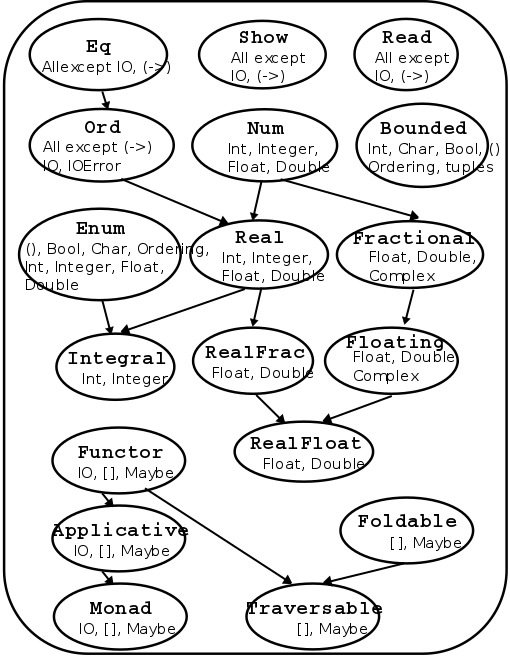
\includegraphics[width=15cm, height=15cm]{image/type-class.png} 
    \caption{Type class \cite{haskell}}
    \label{Type-class}
\end{figure}


\subsection{Inductive Data Types}
Uses a base case then the inductive step as cases of. Multiple arguments. Type constructure

\begin{center}
\begin{tabular}{c}
\begin{lstlisting}[language=Haskell]
data AExp = Atom Int
   | Plus AExp AExp
   | Times AExp AExp

eval (Atom i)    = i
eval (Plus a b)  = eval a + eval b
eval (Times a b) = eval a * eval b
\end{lstlisting}
\end{tabular}
\end{center}

\newpage

\subsection{Trees}
\noindent\textbf{Terminology}
\begin{enumerate}
\item Search tree: All nodes on the left side is less then the parent and opposite on the right side    
\item Out-degree: is how many children it has. Binary trees has out-degree $0-2$
\item root Node: is a parent to any number of children at the top of the hierarchy
\item sub Node: is a parent to any number of children
\item Leaf: is a nod that has no children
\item Node: every element
\item Height: most steps from the root node to a leaf  
\end{enumerate}

\noindent\textbf{Representation}
% https://www.geeksforgeeks.org/tree-traversals-inorder-preorder-and-postorder/
\begin{enumerate}
\item Inorder: (Left, Root, Right)
\item Pre-order: (Root, Left, Right)
\item Post-order: (Left, Right, Root)
\end{enumerate}

\begin{center}
\begin{tabular}{c}
\begin{lstlisting}[language=Haskell]
data FBTree a = Leaf a
   | Node (FBTree a) a (FBTree a)
   deriving (Show)
   
Node (Leaf 1) 5 (Leaf 21)
rootValue :: FBTree a -> a
rootValue (Node _ a _) = a
rootValue (Node x) = x

height :: FBTree a -> Int
height (Leaf _) = 0
height (Node b a c) = 1 + max (height b) (height c)
\end{lstlisting}
\end{tabular}
\end{center}


\newpage
\begin{multicols}{2}
\subsubsection{Binary tree}
\begin{itemize}
  \item Insertion: $O(1)$  ($O(h)$ if search tree)
  \item Delition: $O(n)$   ($O(h)$ if search tree)
  \item Search: $O(n)$  ($O(h)$ if search tree)
  \item Height: $O(n)$ (n nodes)
\end{itemize}

\begin{enumerate}
\item  Full binary tree: has node out-degree either 2 or 0
  worst-case complexity of $O(\log{n})$.
\item  Binary tree: each node has up to an out-degree of 2
\end{enumerate}

\subsubsection{Binary search tree}
\begin{itemize}
  \item Insertion: $O(h)$  ($O(n)$ if search tree)
  \item Delition: $O(h)$
  \item Search: $O(n)$
  \item Height: $O(n)$ (n nodes)
\end{itemize}


\subsubsection{Red and black trees}
\begin{itemize}
  \item Insertion: $O(\log{n})$ % (couldent i be O(n))
  \item Deletion: $O(\log{n})$
  \item Search: $O(\log{n})$ % (couldent i be O(n)), wrong is for BHTree
  \item Element: $O(2^r)$  (rank r) % look it up not shore
  \item Height: $O(2\cdot\log_{2}(n+1))$ (n nodes)
\end{itemize}

Better then a normal binary tree since it balance the tree,
therefor it becomes smaller and more efficient to search in.
One should use red and black tree when there is a large number of nodes, say 50.

Definition: A red-black tree is a binary search tree where every node is
colored either red or black, with the following balancing invariants: 

\begin{enumerate}
\item  No red node has a red parent.
\item  Every path from the root to an empty subtree contains the same.
\item  A red-black tree with n nodes has height at most $2\cdot\log{2}(n+1)$.
\item  there are 4 cases to rebalance (1;4) is similar so is (2;3).
\end{enumerate}

\noindent\textbf{Algorithm}
\begin{enumerate}
\item  Perform a standard binary-search-tree insertion.
\item  Color the new node red.
\item  Rebalance the tree, if there is a red node with a red parent.
\end{enumerate}

\subsubsection{Binomial Trees and heaps}
\begin{itemize}
  \item Insertion: $O(\log{n})$
  \item Search: $O(\log{n})$  (number of trees n)
  \item Element: $2^r$  (rank r, n=1 then r=0)
\end{itemize}

A heap can be used to implement a priority queue, where elements are
added to a pool and assigned a priority. In a min-priority queue,
extraction of an element yields an element with minimum priority.
The smallest node is the root and every child is equal or larger then
its parent.

Binomial Trees is a data structure by linking trees of rank $r-1$ together.
A binomial heap (Vuillemin, 1978) is a list of binomial trees such that
each tree satisfies the min-heap property (hence the root of each tree contains its minimum key);
and the trees have strictly increasing ranks. \newline

\textbf{Terminology}
\begin{enumerate}
\item  Link: putting together two trees.
\item  Merge: putting together two heaps
\item  Binomial Heap: a list (forest!) of Binomial Trees
\item  Binomial Trees have the largest subtree to the left, while Binomial
\end{enumerate}

\textbf{Binomial heaps}
% https://www.youtube.com/watch?v=hbf_h8Ytv04
\begin{enumerate}
\item  Heaps, extracting minimum element in worst case $O(\log{|h|})$
\item  Binomial Trees, The height (here: number of edges on the longest branch) is $r$.
\item  Binomial Trees, There are $2^r$ nodes in the tree.
\item  Binomial Trees, There are $\left(\begin{array}{l}{r}\\{k}\end{array}\right)$ nodes at level k.
  (Hence its name!)
\item  Binomial Trees, The root has r subtrees of ranks $r-1,r-2,\ldots,1,0$.
\item  A binomial heap h has at most $[\lg|h|]+1$ binomial trees.
\item  Inserting a binomial tree into a binomial heap is like addition with base 2.
\item  merging is made with too cases either (case 1) when one is smaller or (case 2) when they are equal
\end{enumerate}

\begin{center}
\begin{tabular}{c}
\begin{lstlisting}[language=Haskell]
  BinoTree = Node Int Int [BinoTree] -- Node rank key (subtrees with decreasing rank)
\end{lstlisting}
\end{tabular}
\end{center}
\end{multicols}
\raggedcolumns


\subsection{Other data types}
\subsubsection{Tables, Stacking and queuing}
\begin{enumerate}
\item  Table: a list of key-value pairs
\item  Stacks: elements accessed in Last-In First-Out (LIFO) order
\item  Queues: elements accessed in First-In First-Out (FIFO) order
\end{enumerate}

\textbf{Table operations}
\begin{center}
\begin{tabular}{c}
\begin{lstlisting}[language=Haskell]
empty :: Table k v
insert :: Eq k => Table k v -> k -> v -> Table k v
exists :: Eq k => Table k v -> k -> Bool
lookup :: Eq k => Table k v -> k -> Maybe v  -- value from key
delete :: Eq k => Table k v -> k -> Table k v
iterate :: Table k v -> (b -> (k, v) -> b) -> b -> b  -- Foldr
keys :: Table k v -> (b -> k -> b) -> b -> b  -- all keys
values :: Table k v -> (b -> v -> b) -> b -> b  -- all values
\end{lstlisting}
\end{tabular}
\end{center}
 

\textbf{Stack operations}
\begin{center}
\begin{tabular}{c}
\begin{lstlisting}[language=Haskell]
-- interface
newtype Stack a = StackImpl [a] -- opaque!

empty :: Stack a
isEmpty :: Stack a -> Bool
push :: a -> Stack a -> Stack a  -- insert
top :: Stack a -> a   -- the first value
pop :: Stack a -> (a,Stack a)  -- take out
\end{lstlisting}
\end{tabular}
\end{center}
 

\textbf{Queue operations}
\begin{center}
\begin{tabular}{c}
\begin{lstlisting}[language=Haskell]
-- interface
newtype Queue a = Q [a] -- opaque

empty :: Queue a  
isEmpty :: Queue a -> Bool
head :: Queue a -> a 
enqueue :: Queue a -> a -> Queue a  -- take out element
dequeue :: Queue a -> Queue a  -- insert element
toList :: Queue a -> [a] 
\end{lstlisting}
\end{tabular}
\end{center}
 
\newpage
\begin{multicols}{2}
\subsubsection{Hashtables}
\begin{itemize}
\item  Key value lookup (an index) 
\item  Array is only define for small index, hash has no limit on avalible keys.
\item  Typically we have n possible keys from set U for a hashtable (which is an array)
  with m slots, where n $\geq$ m.
\item  since there is infinitely many elements and limited amount of key there will be element with
  the  same key, therefor a coalition is created.
\item  Worst-Case Retrieval: time complexity of retrieving a element.
\item  Load Factor: How much data is in the table $\frac{elements}{slots}$
\item  Rehashing: make the hastable more balanced. 
\end{itemize}

\textbf{Collision Resolution by Chaining}
\begin{itemize}
\item Most commonly used collision resolution
\item Let each array slot (also called a bin) hold a list of elements (called a chain).
\item In other words, When collision then add it to a list in that element
\end{itemize}


\textbf{Collision Resolution by Open Addressing}
\begin{itemize}
\item Start with a table with each element is $\perp$ previously used $\Delta$.  
\item Probing: is a function to insert items in a hastable therefore resolves collations
\item Types of probing: \newline
  Linear probing: $f (i)=i$. \newline
  Quadratic probing: $f (i)=c_2\cdot i^2+c_1\cdot i, \; where \; c_2 \neq{0}$. \newline
  Double hashing: $f (i)=i\cdot h'' (i)$, where $h''$ is another hash function. \newline
\item Inserting with Linear Probing: Insert it to the next avalible key 
\item Deleting with Linear Probing: Ignores  $\perp$ and $\Delta$ idex will change.  
\end{itemize}


\subsection{Graphs}
\subsubsection{Types of graphs}
\begin{itemize}
\item list
\item tree
\item forest
\item Directed Acyclic Graph (DAG)  
\end{itemize}

\subsubsection{Treminolage}
\begin{itemize}
\item Node, vertex (plural: vertices)
\item Edge connects two nodes.
\item Self-loop edge from node to itself
\item Adjacent nodes connected by an edge
\item Degree number of edges from or to a node
\item In-degree number of edges to a node
\item Out-degree number of edges from a node
\end{itemize}

\subsubsection{Representation}
\begin{itemize}
\item \textbf{Adjacency Matrix} — a 2-dimensional array A of $0/1$ values, with $A[i, j]$
  containing the number of edges between nodes i and j (undirected graph),
  or from node i to node j \newline
  $+$ edge existence testing in $\theta(1)$ time \newline
  $-$ finding next outgoing edge in $O|V|$ time \newline 
  $+$ compact representation for dense graphs (when $|E|$ is close to $|V|^2$)
\item \textbf{Adjacency List} — a 1-dimensional array Adj of adjacency lists, with 
  Adj[i] containing a list of the nodes adjacent to node i. \newline
  $+$ finding next outgoing edge in $\theta(1)$ time \newline
  $-$ edge existence testing in $O (|V|)$ time \newline
  $+$ compact representation for sparse graphs (when $|E|$ is much smaller than $|V|^2$)
\item \textbf{Edge List} — a list of tuples, (i, j), for each edge (i, j) (plus a list of the nodes). \newline
  $-$ edge existence test in $\theta(|E|)$. \newline
  $-$ finding next outgoing edge in $O (|E|)$ (unless appropriately sorted). \newline
  $+$ compact representation for sparse graphs (when $|E|$ is much smaller than $|V|^2$)
\end{itemize}


\subsubsection{topological sort}
A topological sort is a linear ordering of all the nodes in a directed acyclic. \newline

\noindent\textbf{Algorithm}
\begin{enumerate}
\item Select a node with in-degree 0.
\item Output it.
\item Remove it.
\item Repeat (from 1) until no nodes are left.
\end{enumerate}
Total running time is $\theta(|V|+|E|)$.

\subsubsection{Graph Traversals}
\begin{itemize}
\item Breadth-first search (BFS). Uses a queue for eatch grey node. \newline
  Time complexity: $\theta(|V|+|E|)$  — linear in the size of the graph.
\item Depth-first search (DFS). Uses a stack for eatch (grey) node and has a rest of nodes (white). \newline
  Time complexity: $\theta(|V|+|E|)$  — linear in the size of the graph.
\end{itemize}

\noindent\textbf{Breadth-First Search: Algorithm} \newline
Input: Some node A.
\begin{enumerate}
\item Paint A gray. Paint other nodes white. Add A to an initially empty FIFO queue of gray nodes.
  All grey nodes is in the queue. It is a queue not a stack so first in first out. 
\item Dequeue head node, X. Paint its undiscovered (white) adjacent nodes gray and enqueue them.
  Paint X black. Repeat until queue is empty. For every black node add it to BFS order (black)
\end{enumerate}

\noindent\textbf{Depth-First Search: Algorithm} \newline
Input: Some node A. \newline

\noindent\textbf{DFS(G)}
\begin{enumerate}
\item Paint all nodes white.
\item For each node v in G: if v is (still) white, DFS-Visit(G,v).
  Each subsequent call to DFS-Visit in line 2 is called a restart.
\end{enumerate}

\noindent\textbf{DFS(G)}
\begin{enumerate}
\item Colour v gray.
\item For each node u adjacent to v: if u is white, DFS-Visit(G,u).
\end{enumerate}


\subsubsection{Strongly-Connected Components}
\begin{itemize}
\item Strongly connected component (SCC): maximal set of nodes
  where there is a path from each node to each other node.
\item Many algorithms first divide a digraph into its SCCs, then process
  these SCCs separately, and finally combine the sub-solutions.
  (This is not divide \& conquer, since a different algorithm is run on each SCC!)
\item An undirected graph can be decomposed into its connected
\end{itemize}

\begin{enumerate}
\item Enumerate the nodes of G in DFS finish order, starting from any node
\item Compute the transpose G T (that is, reverse all edges)
\item Make a DFS in G T, considering nodes in reverse finish order from
  original DFS
\item Each tree in this depth-first forest is a strongly connected component
\end{enumerate}
\end{multicols}


\section{Important syntax}
\subsection{Let}
\begin{center}
\begin{tabular}{c}
\begin{lstlisting}[language=Haskell]
  let x = 1 in x * 2 == 2
  case x of
  1 -> "Hello"
  2 -> "H"
  3 -> "Hel"

  input: 3 == "Hel"
  
  # other examples
  let f x y = x + 3 >= y + 3.1 in f 1 1 == False

  f x = let g z = z+1 in g (g x)
  f 1 == 3
  
\end{lstlisting}
\end{tabular}
\end{center}
 
\begin{center}
\begin{tabular}{c}
\begin{lstlisting}[language=Haskell]
:t div
div :: Integral a => a -> a -> a
  
:t (/)
(/) :: Fractional a => a -> a -> a
\end{lstlisting}
\end{tabular}
\end{center}
 

\subsection{IO}
\textbf{monads}
Is used to return an IO and uses a operation \emph(>>=) that replaces \emph{do-notation}
\begin{center}
\begin{tabular}{c}
\begin{lstlisting}[language=Haskell]
class Monad m where
  (>>=) :: m a -> (a -> m b) -> m b
  return :: a -> m a
\end{lstlisting}
\end{tabular}
\end{center}


\section{Sorting Algorithms}
\begin{enumerate}
\item Insertion Sort: One at a time
\item Bubble Sort: sort in order two a time starting from left and work to the right side.
\item Merge Sort: Divide and Conquer, split into even pies and sort them and then merge/sort again. 
\item Quicksort: Divide and Conquer, takes a pivot to spit smaller and larger.
\end{enumerate}
 \newpage
%\input{growing-trees/growing-trees} \newpage
%\input{knots/knots} \newpage
%\input{milling/milling} \newpage
%\input{tree-archive/tree-archive} \newpage


\end{document}
